We requested an expert review from UI/UX professional Andrea Curley. The goal of this review is to evaluate the user interface of Magpie, rate its user-friendliness in regards to UI/UX general guidelines.\\
The expert review was conducted online through a videoconference meeting on Teams and took the following form:
\begin{enumerate}
    \item Presentation of Magpie
    \item Free-roaming of the application by Professor Curley
    \item Questionnaire
    \item Discussion \& end of review
\end{enumerate}
The questionnaire includes questions on visual design, information architecture, data quality \& integration, technical performance, compliance and overall assessment of Magpie as shown in Table 2.3. The review provided very valuable insights on Magpie's workflow, user interface and technical components. These were the main takeaways:\\ \\
\textbf{Landing Page: }
Upon loading Magpie, Professor Curley was directly taken to the mapview, which was not supposed to happen. After the review, we investigated the cause of this event and uncovered a bug in the authentication which we have been working on. Following this event, she suggested creating a landing page or some sort of introduction to ease the user into discovering Magpie.\\ \\
\textbf{Onboarding: }
Due to the bug explained above, the onboarding did not automatically start as it should have upon login. Nevertheless, Professor Curley said that the user may want to intuitively press on the elements being highlighted during the tutorial, as she tried to do. This adds to the feedback received during casual testing for the implementation of this feature. Unfortunately, due to a technical limitations we are not able to solve it, only provide make certain changes to dissuade the user of doing so.\\
In addition, Professor Curley suggested there should be an option to exit the tutorial at any time for users who don't want to sit through it. Lastly, the tutorial shoud be more visually striking and engaging in order to leave a lasting impression on the user.\\ \\
\textbf{Dashboard \& Map: }
Currently, the hierarchy of items on the dashboard does not make sense to the average, and is not intuitive to use. All the amenities are displayed when only one is selected (as shown in figure 3.3) and their count displays zero, which the user might interpret as there are zero other amenities in the area in addition to the one I selected.\\
The icons on the map are not visible enough, and zooming in \& out on the map may not be intuitive to the range of users and devices. Adding zoom buttons could help bridge that gap. \\
Currently, Professor Curley noted that there is a disconnect between the map and the dashboard whereas they should be looked as one. She suggested adding amenity icons to the dashboard to help bridge that gap.\\ \\
\begin{figure}
    %\fbox{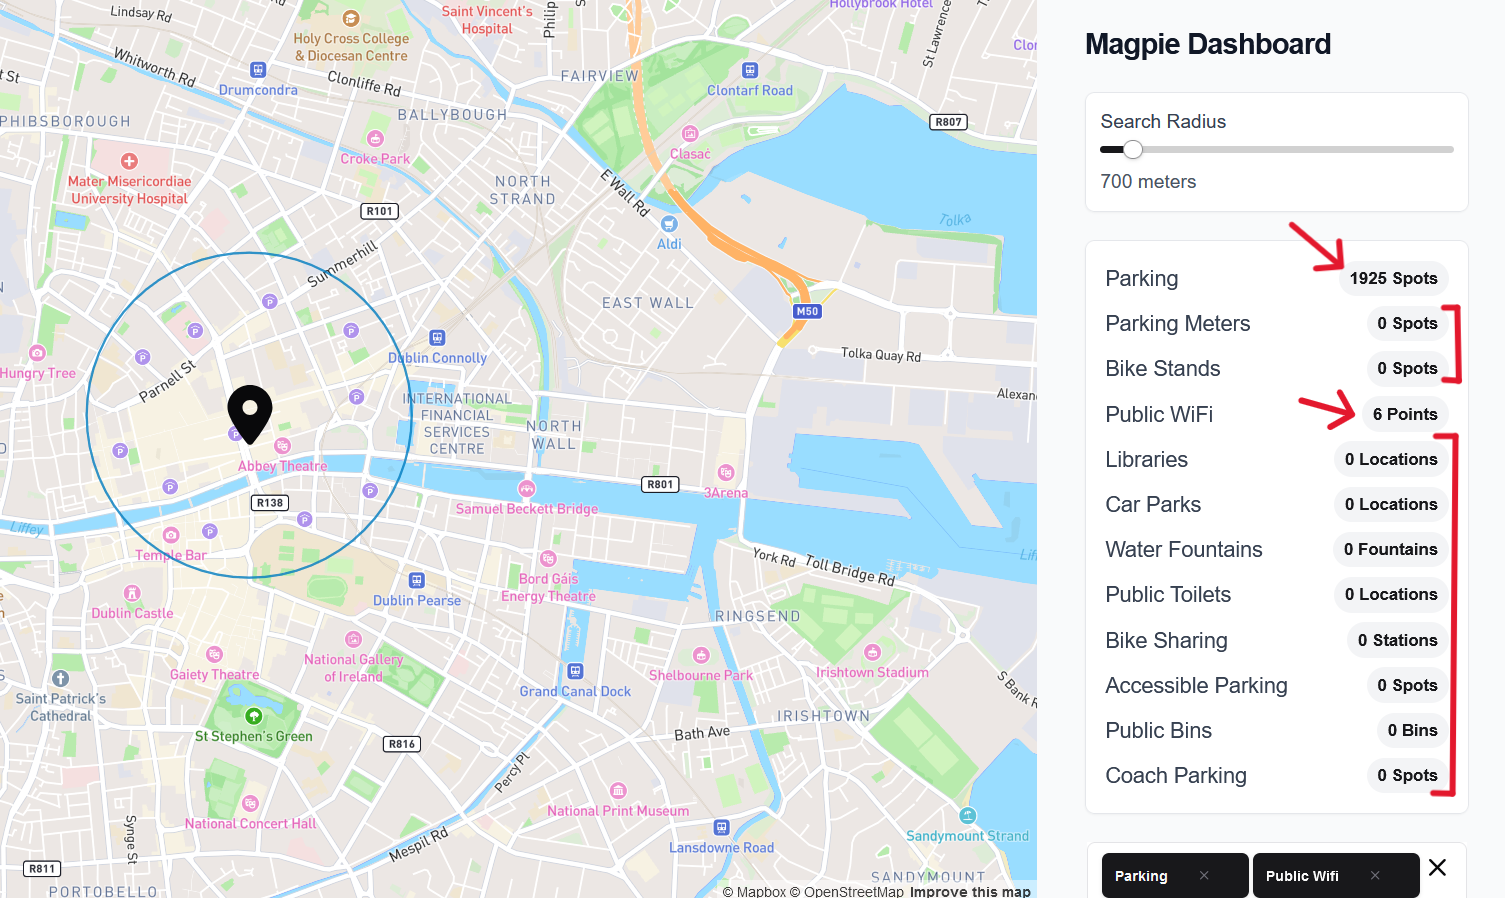
\includegraphics[width=\textwidth]{Figures/fig12.png}}
    \caption{Current dashboard \& map when 2 amenities are selected}
    \label{fig:plot12}
\end{figure}
\textbf{Filters: }
If there are no amenities found in the radius of search, a message should pop up to tell the user so. Currently, it is not very clear if there are amenities present in the chosen area especially due to the small size \& faded color of the icons. \\ \\
\textbf{Log in/sign up: }
When trying to log in with credentials that don't exist, the system should return a proper error such as "username doesn't exist". Log out and account sign up went smoothly. Professor Curley questioned the benefits of logging for Magpie, to which we stated:
Magpie was conceived with the idea of providing a service to working professionals; therefore logging in will allow the implementation of further features such as safeguarding their previous searches, storing exported reports, connecting with other members of your organization and much more.\\ \\
\begin{figure}
    \centering
    %\fbox{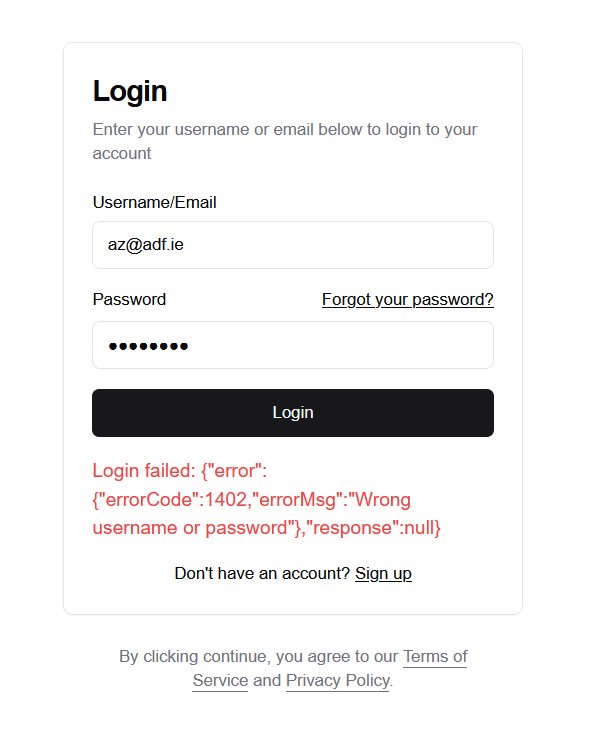
\includegraphics[width=\textwidth]{Figures/fig16.png}}
    \caption{Current error when inputting non-existant username and password}
    \label{fig:plot16}
\end{figure}
\textbf{Overall: }
To resume, Professor Curley found our interface sleek and minimalistic. However, she suggested that if we want to remain with this style, we need to ensure there is as little room as possible for ambiguity and confusion. The user needs to find it easy to move from one feature to another and understand the triggers. Currently, Magpie looks so sleek that the user may not be able to see what they want.\\ \\

\textbf{Survey response}
Below are the answers to the expert review survey in table 3.1. The number next to each multiple choice answer refers to the rating, 1 being the worst and 5 being the best. The response to the survey help complement the oral feedback received during the expert review and provide some quantitative data as a baseline for the next evaluation. The two open-ended questions, to which she asked us to elaborate further, will help us review future open-ended questions and ensure they give enough information for the user to answer.